The exact (average) force we find for a moving particle is:
\begin{align*}
	F &= \frac{1}{2}\hbar k |\Omega_0|^2 \frac{\gamma}{(\omega_0 - \omega + \bm{k}\cdot\bm{v})^2 + \gamma'\ ^2}
\end{align*}
We now seek to calculate the net force applied by a our two lasers that are incident from different directiions:
\begin{align*}
	F_+ &= \frac{1}{2}\hbar k |\Omega_0|^2 \frac{\gamma}{(\omega_0 - \omega + kv)^2 + \gamma'\ ^2} \\
	F_- &= -\frac{1}{2}\hbar k |\Omega_0|^2 \frac{\gamma}{(\omega_0 - \omega - kv)^2 + \gamma'\ ^2}
\end{align*}
We now assume that the detuning is much greater than the doppler shift $|\omega - \omega_0| \gg kv$, so $(\omega_0 - \omega \pm kv)^2 \approx \delta^2 \pm 2\delta kv$. Therefore:
\begin{align*}
	F_\pm &= \pm\frac{1}{2}\hbar k |\Omega_0|^2 \frac{\gamma}{\delta^2 + \gamma'\ ^2}\frac{1}{1\pm \frac{2\delta kv}{\delta^2 + \gamma'\ ^2}} \\
	F_\pm &= \pm\frac{1}{2}\hbar k |\Omega_0|^2 \frac{\gamma}{\delta^2 + \gamma'\ ^2}\left(1\mp \frac{2\delta kv}{\delta^2 + \gamma'\ ^2}\right) \\
	F_\pm &= \pm F_0 - \frac{1}{2}\beta v
\end{align*}
Where:
\begin{align*}
	\beta &= 2\hbar k^2|\Omega_0|^2 \frac{\gamma}{(\delta^2 + \gamma'\ ^2)^2} \delta &
	F_0 &= \frac{1}{2}\hbar k |\Omega_0|^2 \frac{\gamma}{\delta^2 + \gamma'\ ^2}
\end{align*}
So our net force is then:
\begin{align*}
	F &= F_+ + F_- \\
	F &= -\beta v
\end{align*}
So we see we have a damping force. Additionally in practical experiments, as the atom cools, we would decrease the detuning to increase the effect of doppler cooling.

We now naturally wonder how cool can our Doppler cooling get. The key to understanding this is to understand what heating process counterbalances our cooling.
In fact the spontaneous emission process involves a random recoil, despite the fact it is our primary cooling process, it will also be our heating process.
In theremal equilibrium we know our heating and cooling rates will be equal. Our heating rate will be $\frac{(\hbar k)^2}{2M} \rho_{22}\gamma_2$, while the cooling rate is $\expval{\beta v^2}$. So in equilibrium:
\begin{align*}
	\frac{(\hbar k)^2}{2M} \rho_{22} \gamma_2 &= \expval{\beta v^2} \\
	\frac{(\hbar k)^2}{2M} \rho_{22} \gamma_2 &= \beta \frac{k_B T}{M} \\
	\frac{(\hbar k)^2}{2} \rho_{22} \gamma_2 &= \beta k_B T \\
	\frac{(\hbar k)^2}{2} \gamma_2 \frac{|\Omega_0|^2 \gamma}{\gamma_2(\delta^2 + \gamma'\ ^2)} &= k_B T 2\hbar k^2 \frac{|\Omega_0|^2 \gamma \delta}{(\delta^2 +\gamma'\ ^2)^2} \\
	k_B T &= \frac{\hbar}{4} \frac{\delta^2 + \gamma'\ ^2}{\delta} \\
	k_B T &= \frac{\hbar\gamma'}{2} \frac{\delta^2 + \gamma'\ ^2}{2|\delta|\gamma'}
\end{align*}
So:
\begin{align*}
	k_B T &> \frac{\hbar\gamma'}{2} \\
	T_D &= \frac{\hbar\gamma'}{2k_B}
\end{align*}
When first trying to verify this, experiments with $T_D \approx 170 \mu K$ yielded a temperature with $40 \mu K$! This was seen by multiple experiments, and took nearly a year to understand. The explination will be covered in the next lecture.

We already have a cooling force, but we also need to have a trapping force to keep the atoms in place. This can be done with a magneto optic trap.
\subsection{Another perspective}
We have so far looked at these mechanical effects from the perspective of momentum conservation. We ill now look at this from the perspective of dispersive, gradient and dipole forces. Starting from our interaction Hamiltonian:
\begin{align*}
	V &= -\bm{\mu}\cdot\bm{E} &
	\hat{\bm{F}} &= \partial_t \bm{p} \\
	\hat{\bm{F}} &= \frac{1}{i\hbar} [\bm{p}, V] &
	\hat{\bm{F}} &= -\del V
\end{align*}
So our average force is:
\begin{align*}
	\bm{F} &= \expval{\hat{\bm{F}}} \\
	\bm{F} &= -\expval{\del V}
\end{align*}
We now quickly express our potential explicitly:
\begin{align*}
	V &= \frac{\hbar}{2}\Omega_0\sigma_+ + \text{h.c.} &
	\sigma_+ &= \ket{2}\bra{1} \\
	\Omega_0(\bm{r}) &= -\frac{\mu E(\bm{r})}{\hbar} e^{i\phi(\bm{r})} & 
	\Omega_0(\bm{r}) &= |\Omega_0(\bm{r})|e^{i\phi(\bm{r})}
\end{align*}
So:
\begin{align*}
	F &= -\frac{\hbar}{2}\del \Omega_0\expval{\sigma_+} + \text{c.c.} \\
	\expval{\sigma_+} &= \rho_{12} \\
	\expval{\sigma_+} &= -\frac{\Omega_0^*}{2} \frac{1}{\delta + i\gamma} \frac{\delta^2 + \gamma^2}{\delta^2 + \gamma'\ ^2} \\
	\del \Omega_0 &= e^{i\phi}\del |\Omega_0| + i|\Omega_0| e^{i\phi} \del \phi \\
	\del \Omega_0 &= \Omega_0 \left(\frac{\del|\Omega_0|}{|\Omega_0|} + i\del\phi\right) \\
	\bm{F} &= \frac{\hbar}{4}|\Omega_0|^2 \frac{1}{\delta + i\gamma}\frac{\delta^2 + \gamma^2}{\delta^2 + \gamma'\ ^2} \left(\frac{\del|\Omega_0|}{|\Omega_0|} + i\del\phi\right) + \text{c.c.} \\
	\bm{F} &= \frac{\hbar}{4}|\Omega_0|^2 \frac{\delta^2 + \gamma^2}{\delta^2 + \gamma'\ ^2}\left(\frac{-i\gamma}{\delta^2 + \gamma^2} + \frac{\delta}{\delta^2 + \gamma^2}\right) \left(\frac{\del|\Omega_0|}{|\Omega_0|} + i\del\phi\right) + \text{c.c.} \\
	\bm{F} &= \frac{\hbar}{2}|\Omega_0|^2 \frac{\delta^2 + \gamma^2}{\delta^2 + \gamma'\ ^2}\left(\frac{\gamma}{\delta^2 + \gamma^2} \del\phi + \frac{\delta}{\delta^2 + \gamma^2} \frac{\del|\Omega_0|}{|\Omega_0|}\right) \\
	\bm{F} &= \frac{\hbar}{2}|\Omega_0|^2 \frac{1}{\delta^2 + \gamma'\ ^2}\left(\gamma\del\phi + \delta\frac{\del|\Omega_0|}{|\Omega_0|}\right)
\end{align*}
This force has two components, a dissipative force related to $\del\phi$ and a dispersive force related to $\del|\Omega_0|$.
\begin{align*}
	\bm{F}_\text{diss} &= \frac{\hbar}{2}|\Omega_0|^2 \frac{\gamma}{\delta^2 + \gamma'\ ^2}\del\phi \\
	\bm{F}_\text{disp} &= \frac{\hbar}{2}|\Omega_0|^2 \frac{\delta}{\delta^2 + \gamma'\ ^2}\frac{\del|\Omega_0|}{|\Omega_0|} \\
	\bm{F}_\text{disp} &= \frac{\hbar}{4} \frac{\delta}{\delta^2 + \gamma'\ ^2}\del |\Omega_0|^2
\end{align*}
We know for a plane wave $\del|\Omega_0| = 0$ and $\del\phi = \bm{k}$, so for a plane wave:
\begin{align*}
	\bm{F} &= \frac{\hbar}{2}\bm{k} |\Omega_0|^2 \frac{\gamma}{\delta^2 + \gamma'\ ^2}
\end{align*}
Which is what we derived before, so our dissipative force is the force we found for spontaneous emission/absorption.

If we work with a beam of spoot size $~a$, then we will have:
\begin{align*}
	\bm{F}_\text{disp} &\approx \frac{\hbar}{4} \frac{\delta}{\delta^2 + \gamma'\ ^2}\frac{|\Omega_0|^2}{a}
\end{align*}
If we instead look at writing our force in terms of a potential we can say that:
\begin{align*}
	\bm{F}_\text{disp} &= \frac{\hbar}{4} \frac{\delta}{\delta^2 + \gamma^2 + \frac{|\Omega_0|^2}{2}}\del |\Omega_0|^2 \\
	\bm{F}_\text{disp} &= - \del V_\text{opt} \\
	V_\text{opt} &= -\frac{\hbar\delta}{2}\ln \left(1 + \frac{1}{2}\frac{|\Omega_0|^2}{\delta^2 + \gamma^2}\right)
\end{align*}
If we are far off resonance, $\delta \gg \gamma_3$ and $\delta \gg \Omega_0$, then:
\begin{align*}
	V_\text{opt} &\approx -\frac{\hbar\delta}{2}\frac{1}{2}\frac{|\Omega_0|^2}{\delta^2} \\
	V_\text{opt} &\approx -\frac{\hbar}{4}\frac{|\Omega_0|^2}{\delta}
\end{align*}
Which is the optical stark shift. This can be used to create optical tweezers which hold particles in place using a spatially varying intensity.
Additionaly, this can be used to create an optical latice with a periodic potential, where atoms are trapped in one of many potential wells.
\begin{figure*}[h!]
	\centering
	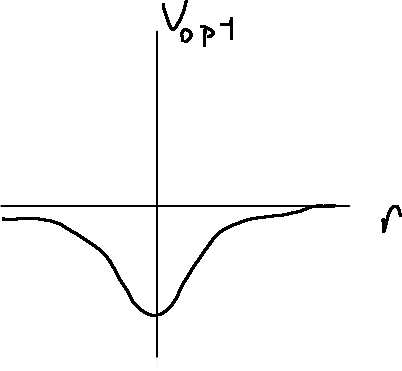
\includegraphics[width=10cm]{images/12-03-1.png}
	\caption*{Potential for Optical tweezers}
\end{figure*}
\begin{figure*}[h!]
	\centering
	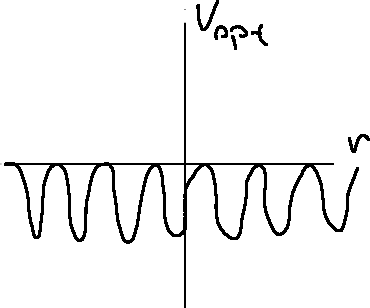
\includegraphics[width=10cm]{images/12-03-2.png}
	\caption*{Potential for Optical lattice}
\end{figure*}
Can we understand the optical stark shift now in terms of conservation of momentum? If our incoming wave is not a plane wave, then we have many wave vectors associated with our beam $\bm{k}$.
If we absorb and re-emit according to different $\bm{k}$s from our beam, then (after some math that is out of scope for what we are looking at), we will see the optical stark shift!
